% Auteur : Samuele Giraudo
% Création : oct. 2013
% Modifications : août 2014 sept 2014 oct. 2014, déc. 2015, jan. 2016
% fev. 2016

\tikzstyle{PointDiag}=[rectangle,draw=Marron!100,fill=Marron!20,
    line width=1pt,minimum width=1cm]
\tikzstyle{TestDiag}=[circle,draw=Bleu!100,fill=Bleu!20,
    line width=1pt]
\tikzstyle{FlecheDiag}=[->,draw=Rouge!80,line width=1pt]
\tikzstyle{CasePile}=[rectangle,draw=GreenYellow!100,fill=GreenYellow!20,
    line width=1pt,minimum width=2.5cm, minimum height=1cm]

%%%%%%%%%%%%%%%%%%%%%%%%%%%%%%%%%%%%%%%%%%%%%%%%%%%%%%%%%%%%%%%%%%%%%%%%
%%%%%%%%%%%%%%%%%%%%%%%%%%%%%%%%%%%%%%%%%%%%%%%%%%%%%%%%%%%%%%%%%%%%%%%%
%%%%%%%%%%%%%%%%%%%%%%%%%%%%%%%%%%%%%%%%%%%%%%%%%%%%%%%%%%%%%%%%%%%%%%%%
\section{Bases}

%%%%%%%%%%%%%%%%%%%%%%%%%%%%%%%%%%%%%%%%%%%%%%%%%%%%%%%%%%%%%%%%%%%%%%%%
%%%%%%%%%%%%%%%%%%%%%%%%%%%%%%%%%%%%%%%%%%%%%%%%%%%%%%%%%%%%%%%%%%%%%%%%
\subsection{Généralités}

%%%%%%%%%%%%%%%%%%%%%%%%%%%%%%%%%%%%%%%%%%%%%%%%%%%%%%%%%%%%%%%%%%%%%%%%
\begin{frame} \frametitle{La notion de programme}
Un \alert{programme} en {\sf C} est avant tout un texte (contenu
dans un {\bf fichier}) qui suit certaines règles (dites de {\bf syntaxe}).
\bigskip
\bigskip

\uncover<2->{
C'est une collection de déclarations et de définitions de fonctions,
de types, de variables globales, assorties de commandes pré-processeur.
\bigskip
\bigskip}

\uncover<3->{
Tout programme possède une {\bf fonction principale} nommée \Code{main}.
C'est par elle que commence l'exécution du programme. On appelle ceci
le \alert{point d'entrée} du programme.}
\end{frame}

%%%%%%%%%%%%%%%%%%%%%%%%%%%%%%%%%%%%%%%%%%%%%%%%%%%%%%%%%%%%%%%%%%%%%%%%
\begin{frame} \frametitle{Compiler un programme}
\alert{Compiler} un programme signifie {\bf traduire} le fichier le
contenant en un langage compréhensible et exécutable par la machine cible.
\medskip

\uncover<2->{
On compile un fichier \Code{Prog.c} par la commande
\begin{center} \Code{gcc -o NOM Prog.c} \end{center}
Ceci produit un exécutable nommé \Code{NOM}.
\bigskip}

\uncover<3->{
On compilera obligatoirement avec les {\bf options} \Code{-ansi},
\Code{-pedantic} et \Code{-Wall} au moyen de la commande
\begin{center} \Code{gcc -o NOM -ansi -pedantic -Wall Prog.c} \end{center}}
\begin{itemize}
    \uncover<4->{
    \item \Code{-ansi -pedantic}~: empêche un programme non compatible
    avec la norme {\sf ANSI C} de compiler~;
    \smallskip}

    \uncover<5->{
    \item \Code{-Wall}~: active tous les messages d'avertissement.}
\end{itemize}
\end{frame}

%%%%%%%%%%%%%%%%%%%%%%%%%%%%%%%%%%%%%%%%%%%%%%%%%%%%%%%%%%%%%%%%%%%%%%%%
%%%%%%%%%%%%%%%%%%%%%%%%%%%%%%%%%%%%%%%%%%%%%%%%%%%%%%%%%%%%%%%%%%%%%%%%
\subsection{Expressions et instructions}

%%%%%%%%%%%%%%%%%%%%%%%%%%%%%%%%%%%%%%%%%%%%%%%%%%%%%%%%%%%%%%%%%%%%%%%%
\begin{frame}\frametitle{Expressions}
Une \alert{expression} est définie récursivement comme étant soit

\begin{enumerate}
    \item une constante~;
    \smallskip

    \uncover<2->{
    \item une variable~;
    \smallskip}

    \uncover<3->{
    \item une combinaison d'expressions et d'opérateurs~;
    \smallskip}

    \uncover<4->{
    \item un appel de fonction qui renvoie une valeur, c.-à-d., de
    type de retour autre que \Code{void}.}
\end{enumerate}
\medskip

\uncover<5->{
Une expression n'est donc rien d'autre qu'un {\bf assemblage de symboles}
qui vérifie des règles {\bf syntaxiques} et {\bf sémantiques}.
\bigskip}

\uncover<6->{
Toute expression possède une \alert{valeur} et un \alert{type}. Le 
processus qui consiste à déterminer la valeur d'une expression se nomme 
l'{\bf évaluation}.
\bigskip}
\end{frame}

%%%%%%%%%%%%%%%%%%%%%%%%%%%%%%%%%%%%%%%%%%%%%%%%%%%%%%%%%%%%%%%%%%%%%%%%
\begin{frame}\frametitle{Expressions}
P.ex., les entités suivantes sont des expressions~:
\begin{multicols}{2}
\begin{itemize}\footnotesize
    \item \Code{0}
    \smallskip
    
    Valeur~: \Code{0}, type~: \Code{int}
    \bigskip
    
    \uncover<2->{
    \item \Code{'a'}
    \smallskip
    
    Valeur~: \Code{97}, type~: \Code{int}
    \bigskip}
    
    \uncover<3->{
    \item \Code{"abc"}
    \smallskip
    
    Valeur~: \Code{"abc"}, type~: \Code{char *}
    \bigskip}
    
    \uncover<4->{
    \item \Code{x}
    \smallskip
    
    Valeur~: \Code{x}, type~: le type de la variable \Code{x}
    \bigskip}
    
    \uncover<5->{
    \item \Code{a == 2}
    \smallskip
    
    Valeur~: \Code{0} ou \Code{1}, type~: \Code{int}
    \bigskip}
    
    \uncover<6->{
    \item \Code{b = 3}
    \smallskip
    
    Valeur~: \Code{3}, type~: \Code{int}
    \bigskip}
    
    \uncover<7->{
    \item \Code{f(5)}
    \smallskip
    
    Valeur~: la valeur renvoyée par \Code{f(5)}, type~: le type de retour
    de \Code{f}
    \bigskip}
    
    \uncover<8->{
    \item \Code{(a == 0) \&\& (b >= 3)}
    \smallskip
    
    Valeur~: \Code{0} ou \Code{1}, type~: \Code{int}
    \bigskip}
    
    \uncover<9->{
    \item \Code{a > 'a' ? a : -a}
    \smallskip
    
    Valeur~: \Code{a} ou \Code{-a}, type~: le type de \Code{a}
    \bigskip}
    
    \uncover<10->{
    \item \Code{1. + 7 * 2}
    \smallskip
    
    Valeur~: \Code{15.}, type~: \Code{float}}
\end{itemize}
\end{multicols}
\end{frame}

%%%%%%%%%%%%%%%%%%%%%%%%%%%%%%%%%%%%%%%%%%%%%%%%%%%%%%%%%%%%%%%%%%%%%%%%
\begin{frame}\frametitle{Instructions}
Une \alert{instruction} est définie récursivement comme étant soit 

\begin{enumerate}
    \item une expression \Code{E;} terminée par un point-virgule~;
    \smallskip
    
    \item un bloc \Code{$\lbrace$ I $\rbrace$} où \Code{I} est une 
    instruction~;
    \smallskip
    
    \item une conditionnelle \Code{if (E) I1 else I2}, où
    \Code{E} est une expression et \Code{I1} et \Code{I2} sont des 
    instructions~;
    \smallskip
    
    \item toute autre construction similaire (\Code{switch}, 
    \Code{while}, \Code{do while}, \Code{for}).
\end{enumerate}
\medskip

\uncover<2->{
À la différence des expressions, c'est souvent l'{\bf effet} d'une
instruction qui est sa raison d'être (et non plus uniquement sa valeur ou
son type).
\medskip}

\uncover<3->{
En effet, une instruction peut p.ex. afficher un élément, allouer
une zone mémoire, lire dans un fichier, {\em etc.} La valeur de
l'expression sous-jacente à l'instruction est d'importance secondaire.}
\end{frame}

%%%%%%%%%%%%%%%%%%%%%%%%%%%%%%%%%%%%%%%%%%%%%%%%%%%%%%%%%%%%%%%%%%%%%%%%
\begin{frame}\frametitle{Instructions}
P.ex., les entités suivantes sont des instructions~:
\begin{multicols}{2}
\begin{itemize}
    \item \Code{;} (instruction vide)
    \bigskip
    
    \item \Code{1;}
    \bigskip
    
    \item \Code{a = b;}
    \bigskip
    
    \item \Code{while (1) {a += 1;}}
    \bigskip
    
    \item \Code{printf("abc\textbackslash n");}
    \bigskip
    
    \item \Code{a++;}
    \bigskip
    
    \item \Code{malloc(64);}
    \bigskip
    
    \item \Code{int tab[64];}
    \bigskip
    
    \item \Code{tab[3] = 9;}
    \bigskip
    
    \item \Code{tab[3];}
    \bigskip
\end{itemize}
\end{multicols}
\end{frame}

%%%%%%%%%%%%%%%%%%%%%%%%%%%%%%%%%%%%%%%%%%%%%%%%%%%%%%%%%%%%%%%%%%%%%%%%
\begin{frame}\frametitle{Expressions à effet de bord}
Une {\bf expression} est à \alert{effet de bord}
(ou encore à \alert{effet secondaire}) si son évaluation modifie
la mémoire.
\bigskip

\uncover<2->{
P.ex., 
\begin{multicols}{2}
\begin{itemize}
    \item \Code{0}, 
    \item \Code{'c'}, 
    \item \Code{(a + 21) <\,< 3},
    \item \Code{tab[8]},
\end{itemize}
\end{multicols}
ne sont pas a effet de bord.
\medskip}

\uncover<3->{
En revanche, 
\begin{multicols}{2}
\begin{itemize}
    \item \Code{a = 31}, 
    \item \Code{printf("abc\textbackslash n")},
    \item \Code{char c},
    \item \Code{malloc(64)},
\end{itemize}
\end{multicols}
sont à effet de bord.}
\end{frame}

%%%%%%%%%%%%%%%%%%%%%%%%%%%%%%%%%%%%%%%%%%%%%%%%%%%%%%%%%%%%%%%%%%%%%%%%
\begin{frame}\frametitle{Expressions à effet de bord}
En règle générale, ce sont les éléments suivants dans les expressions
qui produisent des effets de bord~:
\begin{itemize}
    \item les affectations~;
    \item les allocations de mémoire~;
    \item la sollicitation au système de fichiers.
\end{itemize}
\bigskip

\uncover<2->{
En revanche, les éléments suivants dans les expressions ne produisent
pas d'effet de bord~:
\begin{itemize}
    \item lectures de constantes et de variables~;
    \item calculs arithmétiques, logiques ou bit à bit~;
    \item comparaisons.
\end{itemize}}
\end{frame}

%%%%%%%%%%%%%%%%%%%%%%%%%%%%%%%%%%%%%%%%%%%%%%%%%%%%%%%%%%%%%%%%%%%%%%%%
%%%%%%%%%%%%%%%%%%%%%%%%%%%%%%%%%%%%%%%%%%%%%%%%%%%%%%%%%%%%%%%%%%%%%%%%
\subsection{Constructions syntaxiques}

%%%%%%%%%%%%%%%%%%%%%%%%%%%%%%%%%%%%%%%%%%%%%%%%%%%%%%%%%%%%%%%%%%%%%%%%
\begin{frame}[fragile]\frametitle{Blocs}
Un \alert{bloc} est une suite d'instructions délimitée par des accolades.
Il est constitué d'une partie consacrée à la déclaration de variables
et d'une partie consacrée aux instructions.
\medskip

\uncover<2->{
\begin{multicols}{2}
\Code{$\lbrace$} \\
\quad \Code{DECL} \\
\quad \Code{INST} \\
\Code{$\rbrace$}
\medskip

\Code{DECL}~: section de {\bf déclarations}.
\bigskip

\Code{INST}~: section d'{\bf instructions}.
\bigskip
\end{multicols}}
\bigskip

\uncover<3->{
Les parties \Code{DECL} ou \Code{INST} peuvent être vides. 
\bigskip}

\uncover<4->{
Sachant qu'un bloc est une suite d'instructions, il est possible de
placer un bloc dans la section d'instructions d'un bloc et ainsi
d'{\bf imbriquer} plusieurs blocs.}
\end{frame}

%%%%%%%%%%%%%%%%%%%%%%%%%%%%%%%%%%%%%%%%%%%%%%%%%%%%%%%%%%%%%%%%%%%%%%%%
\begin{frame}[fragile]\frametitle{Blocs}
\begin{multicols}{2}
\begin{semiverbatim}\footnotesize
int main() \{
    int b;
    scanf("%d", &b);
    \textcolor{BrickRed}{\{
        int a;
        a = 1 + b;
    \}}
\}
\end{semiverbatim}

La partie rouge est un bloc au sein d'une fonction \Code{main}.
\bigskip

Il y a des règles concernant la visibilité des variables (que nous
verrons plus loin).
\bigskip
\bigskip
\bigskip
\bigskip
\end{multicols}
\bigskip

\begin{multicols}{2}
\begin{semiverbatim}\footnotesize\uncover<2->{
\{
    int a;
    int b;
    scanf(" %d", &a);
    \textcolor{JungleGreen}{\{
        printf("%d\\n", a);
    \}}
    scanf(" %d", &b);
\}}
\end{semiverbatim}
\uncover<2->{Ceci est un bloc constitué d'une section de déclarations
et d'une section d'instructions.
\bigskip

Cette dernière partie contient un bloc (en vert) dont la section de
déclarations est vide.
\bigskip
\bigskip
\bigskip}
\end{multicols}
\end{frame}

%%%%%%%%%%%%%%%%%%%%%%%%%%%%%%%%%%%%%%%%%%%%%%%%%%%%%%%%%%%%%%%%%%%%%%%%
\begin{frame}\frametitle{Opérateur de test {\tt if}}
L'\alert{opérateur de test} se décline en deux versions~:

\begin{multicols}{2}
\Code{if (EXP)} \\
\quad \Code{BLOC}
\bigskip

\Code{if (EXP)} \\
\quad \Code{BLOC\_1} \\
\Code{else} \\
\quad \Code{BLOC\_2}

Ici, \Code{EXP} est une {\bf expression booléenne}~: elle est considérée comme
fausse si elle s'évalue en zéro et comme vraie sinon. De plus, \Code{BLOC},
\Code{BLOC\_1} et \Code{BLOC\_2} sont des blocs d'instructions.
\end{multicols}
\medskip

\uncover<2->{
Diagrammes d'exécution~:
\begin{multicols}{2}
\begin{center}
\scalebox{.65}{
\begin{tikzpicture}
    \node[PointDiag](Debut)at(0,0){\Code{Debut}};
    \node[TestDiag](EXP)at(0,-1.5){\Code{EXP}};
    \node[PointDiag](BLOC)at(0,-3){\Code{BLOC}};
    \node[PointDiag](Fin)at(0,-4){\Code{Fin}};
    \draw[FlecheDiag](Debut)--(EXP);
    \draw[FlecheDiag](BLOC)--(Fin);
    \draw[FlecheDiag](EXP)edge[bend left=60]node[anchor=west]{$= 0$}(Fin);
    \draw[FlecheDiag](EXP)edge[bend right=60]node[anchor=east]{$\ne 0$}(BLOC);
\end{tikzpicture}}
\end{center}
\begin{center}
\scalebox{.65}{
\begin{tikzpicture}
    \node[PointDiag](Debut)at(0,0){\Code{Debut}};
    \node[TestDiag](EXP)at(0,-1.5){\Code{EXP}};
    \node[PointDiag](BLOC_1)at(-2,-3){\Code{BLOC\_1}};
    \node[PointDiag](BLOC_2)at(2,-3){\Code{BLOC\_2}};
    \node[PointDiag](Fin)at(0,-4){\Code{Fin}};
    \draw[FlecheDiag](Debut)--(EXP);
    \draw[FlecheDiag](BLOC_1)edge[bend right=30](Fin);
    \draw[FlecheDiag](BLOC_2)edge[bend left=30](Fin);
    \draw[FlecheDiag](EXP)edge[bend left=30]node[anchor=west]{$= 0$}(BLOC_2);
    \draw[FlecheDiag](EXP)edge[bend right=30]node[anchor=east]{$\ne 0$}(BLOC_1);
\end{tikzpicture}}
\end{center}
\end{multicols}}
\end{frame}

%%%%%%%%%%%%%%%%%%%%%%%%%%%%%%%%%%%%%%%%%%%%%%%%%%%%%%%%%%%%%%%%%%%%%%%%
\begin{frame}\frametitle{Instruction de branchement {\tt switch}}
L'\alert{instruction de branchement} admet la syntaxe

\begin{multicols}{2}
\Code{switch (EXP) $\lbrace$} \\
\quad \Code{case EXP\_1 : INSTR\_1} \\
\quad \Code{case EXP\_2 : INSTR\_2} \\
\quad \Code{...} \\
\quad \Code{case EXP\_N : INSTR\_N} \\
\quad \Code{default : INSTR\_D} \\
\Code{$\rbrace$}

Ici, \Code{EXP}, \Code{EXP\_1}, \Code{EXP\_2}, \dots, \Code{EXP\_N} sont
des expressions qui s'évaluent en des entiers.
\medskip

Les \Code{INSTR\_1}, \Code{INSTR\_2}, \dots, \Code{INSTR\_N} et
\Code{INSTR\_D} sont des suites d'instructions.
\end{multicols}

\uncover<2->{
L'exécution de cette instruction se passe ainsi.
Soit \Code{i} le plus petit entier (s'il existe) tel que
les évaluations de \Code{EXP} et \Code{EXP\_i} sont égales.
Les instructions \Code{INSTR\_i}, \dots, \Code{INSTR\_N}
ainsi que \Code{INSTR\_D} sont exécutées.
\bigskip}

\uncover<3->{
La ligne \Code{default : INSTR\_D} est facultative.
Si elle est présente, \Code{INSTR\_D} est toujours exécutée.}
\end{frame}

%%%%%%%%%%%%%%%%%%%%%%%%%%%%%%%%%%%%%%%%%%%%%%%%%%%%%%%%%%%%%%%%%%%%%%%%
\begin{frame}\frametitle{Instruction de branchement {\tt switch}}
On s'impose de terminer chaque \Code{INSTR\_j} et \Code{INSTR\_D} par le
mot-clé \Code{break}. 
\medskip

Ceci permet de n'exécuter que le \Code{INSTR\_i} tel que les évaluations 
de \Code{EXP} et \Code{EXP\_i} sont égales. Dans ce cas, \Code{INSTR\_D}
n'est exécuté que si aucun des \Code{EXP\_i} ne l'a été.
\bigskip

On obtient ainsi le diagramme d'exécution
\begin{center}
\scalebox{.65}{
\begin{tikzpicture}
    \node[PointDiag](Debut)at(0,1){\Code{Debut}};
    \node[TestDiag](EXP)at(0,-.5){\Code{EXP}};
    \node[PointDiag](INSTR_1)at(-6,-3){\Code{INSTR\_1}};
    \node[PointDiag](INSTR_2)at(-3,-3){\Code{INSTR\_2}};
    \node at(0,-3){\begin{math}\dots\end{math}};
    \node[PointDiag](INSTR_N)at(3,-3){\Code{INSTR\_N}};
    \node[PointDiag](INSTR_D)at(6,-3){\Code{INSTR\_D}};
    \node[PointDiag](Fin)at(0,-5){\Code{Fin}};
    \draw[FlecheDiag](Debut)--(EXP);
    \draw[FlecheDiag](INSTR_1)edge[bend right=30](Fin);
    \draw[FlecheDiag](INSTR_2)edge[bend right=30](Fin);
    \draw[FlecheDiag](INSTR_N)edge[bend left=30](Fin);
    \draw[FlecheDiag](INSTR_D)edge[bend left=30](Fin);
    \draw[FlecheDiag](EXP)edge[bend right=30]node[anchor=east]
        {$= \Code{EXP\_1}$}(INSTR_1);
    \draw[FlecheDiag](EXP)edge[bend right=30]node[anchor=east]
        {$= \Code{EXP\_2}$}(INSTR_2);
    \draw[FlecheDiag](EXP)edge[bend left=30]node[anchor=west]
        {$= \Code{EXP\_N}$}(INSTR_N);
    \draw[FlecheDiag](EXP)edge[bend left=30]node[anchor=west]
        {$\ne \Code{EXP\_i}, 1 \leq \Code{i} \leq \Code{N}$}(INSTR_D);
\end{tikzpicture}}
\end{center}
\end{frame}

%%%%%%%%%%%%%%%%%%%%%%%%%%%%%%%%%%%%%%%%%%%%%%%%%%%%%%%%%%%%%%%%%%%%%%%%
\begin{frame}\frametitle{Instruction itérative {\tt while}}
L'\alert{instruction itérative} \Code{while} admet la syntaxe

\begin{multicols}{2}
\Code{while (EXP)} \\
\quad \Code{BLOC}
\bigskip

Ici, \Code{EXP} est une expression booléenne et \Code{BLOC}
est un bloc d'instructions.
\end{multicols}
\bigskip

\uncover<2->{
Diagramme d'exécution~:
\begin{center}
\scalebox{.75}{
\begin{tikzpicture}
    \node[PointDiag](Debut)at(0,0){\Code{Debut}};
    \node[TestDiag](EXP)at(0,-1.5){\Code{EXP}};
    \node[PointDiag](BLOC)at(-2,-3){\Code{BLOC}};
    \node[PointDiag](Fin)at(2,-3){\Code{Fin}};
    \draw[FlecheDiag](Debut)--(EXP);
    \draw[FlecheDiag](EXP)edge[bend left=60]node[anchor=west]{$= 0$}(Fin);
    \draw[FlecheDiag](EXP)edge[bend right=60]node[anchor=east]{$\ne 0$}(BLOC);
    \draw[FlecheDiag](BLOC)edge[bend right=20](EXP);
\end{tikzpicture}}
\end{center}}
\end{frame}

%%%%%%%%%%%%%%%%%%%%%%%%%%%%%%%%%%%%%%%%%%%%%%%%%%%%%%%%%%%%%%%%%%%%%%%%
\begin{frame}\frametitle{Instruction itérative {\tt do while}}
L'\alert{instruction itérative} \Code{do while} admet la syntaxe

\begin{multicols}{2}
\Code{do} \\
\quad \Code{BLOC} \\
\Code{while (EXP);}
\bigskip

Ici, \Code{EXP} est une expression booléenne et \Code{BLOC}
est un bloc d'instructions.
\end{multicols}
\bigskip

\uncover<2->{
Diagramme d'exécution~:
\begin{center}
\scalebox{.75}{
\begin{tikzpicture}
    \node[PointDiag](Debut)at(0,0){\Code{Debut}};
    \node[PointDiag](BLOC)at(0,-1){\Code{BLOC}};
    \node[TestDiag](EXP)at(0,-2.5){\Code{EXP}};
    \node[PointDiag](Fin)at(0,-4){\Code{Fin}};
    \draw[FlecheDiag](Debut)--(BLOC);
    \draw[FlecheDiag](BLOC)--(EXP);
    \draw[FlecheDiag](EXP)edge[]node[anchor=west]{$= 0$}(Fin);
    \draw[FlecheDiag](EXP)edge[bend right=90]node[anchor=west]{$\ne 0$}(BLOC);
\end{tikzpicture}}
\end{center}}
\end{frame}

%%%%%%%%%%%%%%%%%%%%%%%%%%%%%%%%%%%%%%%%%%%%%%%%%%%%%%%%%%%%%%%%%%%%%%%%
\begin{frame}\frametitle{Instruction itérative {\tt for}}
L'\alert{instruction itérative} \Code{for} admet la syntaxe

\begin{multicols}{2}
\Code{for (EXP\_1 ; EXP\_2 ; EXP\_3)} \\
\quad \Code{BLOC}
\bigskip

Ici, \Code{EXP\_2} est une expression booléenne (le {\bf test}),
\Code{EXP\_1} (l'{\bf initialisation}) et \Code{EXP\_3}
(l'{\bf incrémentation}) sont des expressions et \Code{BLOC}
est un bloc d'instructions.
\end{multicols}
\smallskip

\uncover<2->{
Diagramme d'exécution~:
\begin{center}
\scalebox{.71}{
\begin{tikzpicture}
    \node[PointDiag](Debut)at(0,0){\Code{Debut}};
    \node[PointDiag](EXP_1)at(0,-1){\Code{EXP\_1}};
    \node[TestDiag](EXP_2)at(0,-2.5){\scriptsize\Code{EXP\_2}};
    \node[PointDiag](BLOC)at(2,-4){\Code{BLOC}};
    \node[PointDiag](EXP_3)at(2,-5){\Code{EXP\_3}};
    \node[PointDiag](Fin)at(-2,-5){\Code{Fin}};
    \draw[FlecheDiag](Debut)--(EXP_1);
    \draw[FlecheDiag](EXP_1)--(EXP_2);
    \draw[FlecheDiag](EXP_2)edge[bend left=30]node[anchor=north east]
        {$\ne 0$}(BLOC);
    \draw[FlecheDiag](BLOC)--(EXP_3);
    \draw[FlecheDiag](EXP_3)edge[bend left=30](EXP_2);
    \draw[FlecheDiag](EXP_2)edge[bend right=30]node[anchor=west]{$= 0$}(Fin);
\end{tikzpicture}}
\end{center}}
\end{frame}

%%%%%%%%%%%%%%%%%%%%%%%%%%%%%%%%%%%%%%%%%%%%%%%%%%%%%%%%%%%%%%%%%%%%%%%%
\begin{frame}[fragile]\frametitle{Instruction itérative {\tt for}}\small
\begin{multicols}{2}
\begin{semiverbatim}\small
for (i = 0 ; i < 3 ; ++i) \{
    printf("a");
\}
\end{semiverbatim}
Affiche trois occurrences du caractère \Code{'a'}.
\end{multicols}
%\smallskip

\begin{multicols}{2}
\begin{semiverbatim}\small\uncover<2->{
for (x = lst ; x != NULL ;
        x = x->suiv) \{
    afficher(x->elem);
\}}
\end{semiverbatim}
\uncover<2->{
Parcours une liste simplement chaînée et l'affiche.
La variable \Code{x} est un pointeur sur la cellule courante.}
\end{multicols}
%\smallskip

\begin{multicols}{2}
\begin{semiverbatim}\small\uncover<3->{
for ( ; *str != '\\0'; str++)) \{
    putchar(*str);
\}}
\end{semiverbatim}
\uncover<3->{
Affiche la chaîne de caractères \Code{str}. Il n'y a pas d'initialisation.
L'incrémentation fait pointer \Code{str} sur le prochain caractère.}
\end{multicols}
%\smallskip

\begin{multicols}{2}
\begin{semiverbatim}\small\uncover<4->{
for ( ; *str != '\\0';
        putchar(*str++)) \{
    /* Rien. */
\}}
\end{semiverbatim}
\uncover<4->{
Affiche la chaîne de caractères \Code{str}. Il n'y a pas
d'initialisation. L'affichage est réalisé comme effet de bord
de l'incrémentation.}
\end{multicols}
\end{frame}

%%%%%%%%%%%%%%%%%%%%%%%%%%%%%%%%%%%%%%%%%%%%%%%%%%%%%%%%%%%%%%%%%%%%%%%%
\begin{frame}[fragile]\frametitle{Instructions de court-circuit}
Les \alert{instructions de court-circuit} sont \Code{break} et
\Code{continue}.
\bigskip

\uncover<2->{
L'instruction \Code{break} permet à l'exécution de sortir d'une structure
\Code{switch}, \Code{while}, \Code{do while} ou \Code{for}.
L'exécution continue alors aux instructions qui suivent cette structure.
\bigskip}

\uncover<3->{
L'instruction \Code{continue} permet à l'exécution de sauter à la fin du
bloc \Code{BLOC} d'une structure \Code{while}, \Code{do while} ou 
\Code{for}. L'exécution continue alors à l'évaluation de l'expression 
test.}
\end{frame}

%%%%%%%%%%%%%%%%%%%%%%%%%%%%%%%%%%%%%%%%%%%%%%%%%%%%%%%%%%%%%%%%%%%%%%%%
\begin{frame}[fragile]\frametitle{Instructions de court-circuit}
Dans une boucle \Code{for}, l'instruction \Code{continue}
fait que l'expression d'incrémentation est tout de même évaluée.
\medskip

\begin{multicols}{2}
\begin{semiverbatim}\uncover<2->{
for (i = 1 ; i <= 7 ; ++i) \{
    if (i == 4)
        continue;
    printf("%d ", i);
\}}
\end{semiverbatim}
\uncover<2->{
L'exécution de ces instructions produit sept tours de boucle et 
l'affichage \Code{1 2 3 5 6 7}.
Lorsque \Code{i == 4}, le \Code{continue} relance l'exécution à 
l'incrémentation du \Code{for}.}
\end{multicols}
\bigskip

\uncover<3->{Ce n'est pas le cas pour le \Code{break}.
\medskip}

\begin{multicols}{2}
\begin{semiverbatim}\uncover<4->{
for (i = 1 ; i <= 7 ; ++i) \{
    if (i == 4)
        break;
    printf("%d ", i);
\}}
\end{semiverbatim}
\uncover<4->{
L'exécution de ces instructions produit quatre tours de boucle
et l'affichage \Code{1 2 3}.
Lorsque \Code{i == 4}, le \Code{break} fait sortir de la
boucle et \Code{i} vaut \Code{4}.}
\end{multicols}
\end{frame}

%%%%%%%%%%%%%%%%%%%%%%%%%%%%%%%%%%%%%%%%%%%%%%%%%%%%%%%%%%%%%%%%%%%%%%%%
%%%%%%%%%%%%%%%%%%%%%%%%%%%%%%%%%%%%%%%%%%%%%%%%%%%%%%%%%%%%%%%%%%%%%%%%
\subsection{Variables}

%%%%%%%%%%%%%%%%%%%%%%%%%%%%%%%%%%%%%%%%%%%%%%%%%%%%%%%%%%%%%%%%%%%%%%%%
\begin{frame} \frametitle{Variables}
Une \alert{variable} est une entité constituée des cinq éléments suivants~:
\medskip

\begin{multicols}{2}
\begin{enumerate}
    \uncover<2->{\item un identificateur~;}
    \uncover<3->{\item un type~;}
    \uncover<4->{\item une valeur~;}
    \uncover<5->{\item une adresse~;}
    \uncover<6->{\item une portée lexicale.}
\end{enumerate}
\begin{center}
\begin{tikzpicture}
    \uncover<2->{
    \draw[fill=Rouge!30](0,-.5)rectangle node{\small Identificateur}(2,0);}
    \uncover<3->{
    \draw[fill=Orange!30](2,-.5)rectangle node{\small Type}(3,1);}
    \uncover<4->{
    \draw[fill=Bleu!30](0,0)rectangle node{\small Valeur}(2,1);}
    \uncover<5->{
    \node(adr)at(-2,0){\small Adresse};
    \draw(adr)edge[->,bend right=20](0,-.25);}
\end{tikzpicture}
\end{center}
\end{multicols}
\bigskip

\uncover<7->{
{\bf Intuitivement}, c'est une boîte qui peut contenir un objet (valeur) et
qui dispose d'un nom (identificateur).
\smallskip

Une boîte ne peut contenir que des objets d'une certaine sorte (type).
\smallskip

Elle se situe de plus à un endroit bien précis dans la mémoire (adresse)
et elle n'est visible qu'à partir de certains endroits du code
(portée lexicale).}
\end{frame}

%%%%%%%%%%%%%%%%%%%%%%%%%%%%%%%%%%%%%%%%%%%%%%%%%%%%%%%%%%%%%%%%%%%%%%%%
\begin{frame} \frametitle{Identificateurs de variable}
L'\alert{identificateur} d'une variable est un mot commençant par une
lettre ou bien \Code{'\_'}, suivi par un nombre arbitraire de lettres,
chiffres ou \Code{'\_'}.
\bigskip

De plus, aucun identificateur ne peut-être un \alert{mot réservé} du
langage. En voici la liste complète~:
\begin{center}
    \scriptsize
    \begin{tabular}{cccccccc}
        \Code{auto} & \Code{break} & \Code{case} & \Code{char} &
        \Code{const} & \Code{continue} & \Code{default} & \Code{do} \\[.5em]
        \Code{double} & \Code{else} & \Code{enum} & \Code{extern} &
        \Code{float} & \Code{for} & \Code{goto} & \Code{if} \\[.5em]
        \Code{int} & \Code{long} & \Code{register} & \Code{return} &
        \Code{short} & \Code{signed} & \Code{sizeof} & \Code{static} \\[.5em]
        \Code{struct} & \Code{switch} & \Code{typedef} & \Code{union} &
        \Code{unsigned} & \Code{void} & \Code{volatile} & \Code{while}
    \end{tabular}
\end{center}
\bigskip

\uncover<2->{
L'identificateur d'une variable est \alert{attribué à sa déclaration}.}
\end{frame}

%%%%%%%%%%%%%%%%%%%%%%%%%%%%%%%%%%%%%%%%%%%%%%%%%%%%%%%%%%%%%%%%%%%%%%%%
\begin{frame}[fragile] \frametitle{Valeur d'une variable}
La \alert{valeur} d'une variable est la raison pour laquelle celle-ci
existe. Le rôle premier d'une variable étant en effet de contenir une
valeur.
\bigskip

\uncover<2->{
La valeur d'une variable n'est \alert{pas attribuée à sa déclaration}
(elle contient à ce moment là une valeur mais il ne faut rien supposer
dessus).
\medskip}

\uncover<3->{
On accède à la valeur valeur d'une variable par son identificateur.
\bigskip}

\uncover<4->{
On modifie une variable par une {\bf affectation}. L'occurrence de
l'identificateur de la variable se trouve dans ce cas à gauche de
l'opérateur \Code{=}.}
\medskip

\begin{multicols}{2}
\begin{semiverbatim}\uncover<5->{
int num;

num = 23;
num = num + 32;}
\end{semiverbatim}
\bigskip
\bigskip

\uncover<5->{
L'occurrence de \Code{num} en l. 2 est située à gauche du \Code{=}~:
il s'agit d'une affectation. Il y en a deux en ligne $3$~: la $1\iere$
permet de modifier et la $2\ieme$ de lire sa valeur.}
\end{multicols}
\end{frame}

%%%%%%%%%%%%%%%%%%%%%%%%%%%%%%%%%%%%%%%%%%%%%%%%%%%%%%%%%%%%%%%%%%%%%%%%
\begin{frame}[fragile] \frametitle{{\it L}-values et {\it R}-values}
Nous rencontrons une subtilité~: un identificateur \Code{x} de variable 
peut désigner soit~:
\begin{enumerate}
    \item la valeur de la variable \Code{x}, p.ex., dans 
    \Code{x + 16}~;
    \smallskip
    
    \uncover<2->{
    \item soit la variable \Code{x} elle-même, p.ex., dans 
    \Code{x += 8}.}
\end{enumerate}
\medskip

\uncover<3->{
La terminologie de \og{\it L}-value\fg{} (valeur gauche) et 
\og{\it R}-value\fg{} (valeur droite) permet de mettre en évidence cette
différence.
\bigskip}

\uncover<4->{
Une \alert{{\it L}-value} est une expression qui peut se situer dans le 
membre gauche d'une affectation (l'expression peut {\bf recevoir} une 
valeur).
\bigskip}

\uncover<5->{
Une \alert{{\it R}-value} est une expression qui peut se situer dans le 
membre droit d'une affectation (une valeur peut être {\bf lue} depuis
l'expression).
\bigskip}

\uncover<6->{
{\bf Note~:} toute {\it L}-value est une {\it R}-value, mais pas 
l'inverse.}
\end{frame}

%%%%%%%%%%%%%%%%%%%%%%%%%%%%%%%%%%%%%%%%%%%%%%%%%%%%%%%%%%%%%%%%%%%%%%%%
\begin{frame}[fragile] \frametitle{Adresse d'une variable}
L'\alert{adresse} d'une variable est une valeur entière spécifiant la
position de la variable en mémoire.
\bigskip

\uncover<2->{
L'adresse d'une variable est \alert{attribuée à sa déclaration} par
le système à l'{\bf exécution}. Elle ne peut pas être choisie par le
programmeur ni être modifiée.
\bigskip}

\uncover<3->{
On accède à l'adresse d'une variable par son identificateur précédé
de l'opérateur \Code{$\&$}.}

\begin{multicols}{2}
\begin{semiverbatim}\uncover<4->{
int num;

printf("%p\\n", &num);}
\end{semiverbatim}
\bigskip
\bigskip
\bigskip

\uncover<4->{
Une $1\iere$ exécution de ces instructions affiche \Sortie{0x7fff6a3014fc}.
Une $2\ieme$ affiche \Sortie{0x7fffbdc357dc}. L'adresse de \Code{num}
varie d'une exécution à l'autre.}
\end{multicols}
\end{frame}

%%%%%%%%%%%%%%%%%%%%%%%%%%%%%%%%%%%%%%%%%%%%%%%%%%%%%%%%%%%%%%%%%%%%%%%%
\begin{frame}[fragile]
    \frametitle{Portée lexicale d'une variable et variables locales}
La \alert{portée lexicale} d'une variable désigne la
{\bf zone du programme} dans laquelle la variable peut être utilisée.
\bigskip

\uncover<2->{
Elle dépend de l'endroit dans lequel elle a été déclarée.
\bigskip}

\uncover<3->{
Sa portée lexicale s'étend aux instructions qui sont situées
après sa déclaration dans le plus petit bloc d'instructions qui
la contient.
\bigskip}

\begin{multicols}{2}
\begin{semiverbatim}\small\uncover<4->{
void f(int x) \{
    int a, b;
    ...
\}

int g(int y, int z) \{
    int c;
    ...
\}}
\end{semiverbatim}
\small
\uncover<4->{
La portée lexicale des variables \Code{a} et \Code{b} s'étend aux
instructions du corps de la fonction \Code{f}.
Elle ne s'étend pas aux instructions du corps de \Code{g}. Les variables
\Code{a} et \Code{b} sont des \alert{variables locales} à la fonction \Code{f}
et invisibles ailleurs.
\smallskip}

\uncover<5->{
Le \alert{paramètre} \Code{x} de \Code{f} a pour portée lexicale uniquement
le corps de \Code{f}.}
\end{multicols}
\end{frame}

%%%%%%%%%%%%%%%%%%%%%%%%%%%%%%%%%%%%%%%%%%%%%%%%%%%%%%%%%%%%%%%%%%%%%%%%
\begin{frame}[fragile]
    \frametitle{Portée lexicale d'une variable et variables locales}
\begin{multicols}{2}
\begin{semiverbatim}
...
int f() \{...\}
...
int taille = 31;
...
int g() \{...\}
...
int main() \{...\}
\end{semiverbatim}
La portée lexicale de la variable \Code{taille} s'étend à tout ce qui
suit sa déclaration dans le programme. Elle est donc visible dans les
fonctions \Code{g} et \Code{main} mais pas dans \Code{f}. Étant donné
qu'elle est déclarée en dehors de toute fonction, elle est qualifiée de
\alert{variable globale}.
\end{multicols}
\bigskip

\uncover<2->{
{\bf Attention}~: l'utilisation de variables globales n'est ni élégante
ni indispensable. Elle est bannie pour ces raisons.
\smallskip

On préfère utiliser des définitions préprocesseur pour représenter
leur valeur.}
\end{frame}

%%%%%%%%%%%%%%%%%%%%%%%%%%%%%%%%%%%%%%%%%%%%%%%%%%%%%%%%%%%%%%%%%%%%%%%%
\begin{frame}[fragile]
\frametitle{Portée lexicale d'une variable et blocs d'instructions}
\begin{multicols}{2}
\begin{semiverbatim}
\{
    int a;
    a = 15;
    printf("%d", a);
\}
printf("%d", a);
\end{semiverbatim}
Il y a erreur de compilation~: la portée
lexicale de la variable \Code{a} s'étend de la l. 2 à la l. 5.
Elle n'est pas visible à la l. 6. Il n'existe
pas de variable identifiée par \Code{a} lorsque la l. 7 est évaluée.
\end{multicols}
\smallskip

\begin{multicols}{2}
\begin{semiverbatim}\small\uncover<2->{
\{
    int a;
    a = 15;
    printf("%d", a);
\}
\{
    printf("%d", a);
\}}
\end{semiverbatim}
\uncover<2->{
De la même manière que dans l'exemple précédent, l'occurrence
du symbole \Code{a} dans le second bloc (l. 7) n'est pas
résolue. Elle se situe dans un bloc qui n'est pas contenu
par celui où le symbole \Code{a} est déclaré.}
\end{multicols}
\end{frame}

%%%%%%%%%%%%%%%%%%%%%%%%%%%%%%%%%%%%%%%%%%%%%%%%%%%%%%%%%%%%%%%%%%%%%%%%
\begin{frame}[fragile]
\frametitle{Portée lexicale d'une variable et blocs d'instructions}
\begin{multicols}{2}
\begin{semiverbatim}
int a;
a = 10;
\{
    printf("%d ", a);
\}
printf("%d\\n", a);
\end{semiverbatim}
\medskip

Ces instructions produisent l'affichage \Sortie{10 10}. En effet, la
variable \Code{a} est visible dans le bloc d'instructions dans lequel
elle est définie, ainsi que dans les blocs d'instructions qui se trouvent
à l'intérieur.
\end{multicols}
\smallskip

\begin{multicols}{2}
\begin{semiverbatim}\small\uncover<2->{
int a;
a = 10;
\{
    int a;
    a = 20;
    printf("%d ", a);
\}
printf("%d\\n", a);}
\end{semiverbatim}
\uncover<2->{
Ces instructions produisent l'affichage \Sortie{20 10}. La variable
identifiée par \Code{a} dans le bloc d'instructions de la l. 3 à
la l. 7 est celle déclarée en l. 4. La variable identifiée par
\Code{a} hors de ce bloc d'instructions est celle déclarée en l. 1.}
\end{multicols}
\end{frame}

%%%%%%%%%%%%%%%%%%%%%%%%%%%%%%%%%%%%%%%%%%%%%%%%%%%%%%%%%%%%%%%%%%%%%%%%
\begin{frame}[fragile]
\frametitle{Portée lexicale d'une variable et blocs d'instructions}
Comparons les instructions
\begin{multicols}{2}
\begin{semiverbatim}\small
int a;
a = 10;
\{
    int a;
    a = 20;
    printf("%d ", a);
\}
printf("%d\\n", a);
\end{semiverbatim}
\begin{semiverbatim}\small
int a;
a = 10;
\{
    a = 20;
    printf("%d ", a);
\}
printf("%d\\n", a);
\end{semiverbatim}
\end{multicols}
\bigskip

\uncover<2->{
Dans le cas de gauche (déjà vu), l'affectation \Code{a = 20} n'a d'effet
que sur la variable \Code{a} déclarée à l'intérieur du bloc. Ceci
affiche \Sortie{20 10}.
\bigskip}

\uncover<3->{
En revanche, les instructions de droite affichent \Sortie{20 20} car
il n'y a pas de déclaration de \Code{a} dans le bloc. L'affectation
\Code{a = 20} modifie la variable \Code{a} déclarée en l. 1.}
\end{frame}

%%%%%%%%%%%%%%%%%%%%%%%%%%%%%%%%%%%%%%%%%%%%%%%%%%%%%%%%%%%%%%%%%%%%%%%%
%%%%%%%%%%%%%%%%%%%%%%%%%%%%%%%%%%%%%%%%%%%%%%%%%%%%%%%%%%%%%%%%%%%%%%%%
\subsection{Fonctions et pile}

%%%%%%%%%%%%%%%%%%%%%%%%%%%%%%%%%%%%%%%%%%%%%%%%%%%%%%%%%%%%%%%%%%%%%%%%
\begin{frame}[fragile] \frametitle{Fonctions}
Une \alert{fonction} est constituée
\begin{enumerate}
    \item d'un identificateur (qui suit les mêmes contraintes que ceux des
    variables)~;
    \item d'une signature (la liste de ses paramètres et de leurs types)~;
    \item d'un type de retour (le type de la valeur renvoyée par la fonction)~;
    \item d'instructions (qui forment le corps de la fonction).
\end{enumerate}
\bigskip

\uncover<2->{
La ligne constituée du type de retour, de l'identificateur et
de la signature d'une fonction est son {\bf prototype}.
\bigskip}

\uncover<3->{P.ex.,}
\begin{semiverbatim}\uncover<3->{
int produit(int a, int b, int c) \{
    return a * b * c;
\}}
\end{semiverbatim}
\uncover<3->{
est une fonction d'identificateur \Code{produit}, de signature
\Code{(int a, int b, int c)} et de type de retour \Code{int}.}
\end{frame}

%%%%%%%%%%%%%%%%%%%%%%%%%%%%%%%%%%%%%%%%%%%%%%%%%%%%%%%%%%%%%%%%%%%%%%%%
\begin{frame}[fragile] \frametitle{Définition {\em vs} déclaration}
La \alert{définition} d'une fonction consiste à fournir tous ses 
constituants.
\medskip

\uncover<2->{
La \alert{déclaration} d'une fonction consiste à fournir son
\alert{prototype}.
\medskip}

\uncover<3->{
Déclarer une fonction est utile si l'on souhaite s'en servir avant de
l'avoir définie.
\smallskip}

\uncover<4->{
Voici un exemple~:}
\begin{multicols}{2}
\begin{semiverbatim}\small\uncover<4->{
#include <stdio.h>


/* Declarations. */
void flop(int nb);
void flip(int nb);

/* Definitions. */
int main() \{
    flip(10);
    return 0;
\}

void flip(int nb) \{
    if (nb >= 1) \{
        printf("flip\\n");
        flop(nb - 1);
    \}
\}
void flop(int nb) \{
    if (nb >= 1) \{
        printf("flop\\n");
        flip(nb - 1);
    \}
\}}
\end{semiverbatim}
\end{multicols}
\end{frame}

%%%%%%%%%%%%%%%%%%%%%%%%%%%%%%%%%%%%%%%%%%%%%%%%%%%%%%%%%%%%%%%%%%%%%%%%
\begin{frame}[fragile] \frametitle{Paramètres {\em vs} arguments}
Il faut faire attention à bien distinguer les notions de paramètre et
d'argument qui sont deux choses différentes.
\bigskip

\uncover<2->{
On considère la fonction}
\begin{semiverbatim}\uncover<2->{
int produit(int a, int b, int c) \{
    return a * b * c;
\}}
\end{semiverbatim}
\medskip

\uncover<3->{
Les symboles \Code{a}, \Code{b} et \Code{c} de son prototype sont ses
\alert{paramètres}.}
\bigskip
\bigskip

\uncover<4->{
Lors de l'appel}
\begin{semiverbatim}\uncover<4->{
produit(15, num, -3);}
\end{semiverbatim}
\uncover<4->{
les valeurs \Code{15}, \Code{num} et \Code{-3} sont les \alert{arguments}
de l'appel.
\bigskip}

\uncover<5->{
{\bf Aide-mémoire}~: {\bf p}aramètre $\leftrightarrow$ {\bf p}rototype~;
{\bf a}rgument $\leftrightarrow$ {\bf a}ppel.}
\end{frame}

%%%%%%%%%%%%%%%%%%%%%%%%%%%%%%%%%%%%%%%%%%%%%%%%%%%%%%%%%%%%%%%%%%%%%%%%
\begin{frame}[fragile] \frametitle{Portée lexicale des paramètres}
Les variables locales d'une fonction ont pour portée lexicale la
fonction elle-même (déjà mentionné).
\bigskip

\uncover<2->{
Il en est de même pour ses {\bf paramètres}~: leur portée lexicale est
la fonction elle-même. On peut voir la déclaration des paramètres d'une
fonction dans son en-tête comme une déclaration de variable.
\bigskip}

\begin{multicols}{2}
\begin{semiverbatim}\small\uncover<3->{
int double(int a) \{
    return 2 * a;
\}

int main() \{
    int a;
    a = 10;
    a = double(a + 1);
    return 0;
\}}
\end{semiverbatim}
\uncover<3->{
Il y plusieurs occurrences du symbole \Code{a}.
\smallskip

Celui déclaré dans l'en-tête de \Code{double} a une portée
lexicale qui s'étend de la l. 1 à la l. 3.
\smallskip

Celui déclaré dans le \Code{main} a pour portée lexicale le \Code{main}
tout entier.
\medskip

Ce sont des variables différentes.}
\end{multicols}
\end{frame}

%%%%%%%%%%%%%%%%%%%%%%%%%%%%%%%%%%%%%%%%%%%%%%%%%%%%%%%%%%%%%%%%%%%%%%%%
\begin{frame}[fragile] \frametitle{Pile}
Lors de l'appel d'une fonction, les valeurs de ses arguments sont
\alert{recopiées} dans une zone de la mémoire appelée \alert{pile}.
\bigskip

{\bf Conséquence très importante}~: toute modification des paramètres
dans une fonction ne modifie pas les valeurs des arguments avec lesquels
elle a été appelée.
\bigskip

P.ex.,
\begin{multicols}{2}
\begin{lstlisting}[basicstyle=\ttfamily\scriptsize]
void incr(int a) {
    a = a + 1;
}

int f() {
    int b;
    
    b = 3;
    incr(b);
    printf("%d\n", b);
    return 0;
}
...
f();
\end{lstlisting}
\small
L'appel à \Code{f} en l. 14 produit les configurations de pile
\begin{flushleft}
    \begin{tabular}{ccc}
    \scalebox{.45}{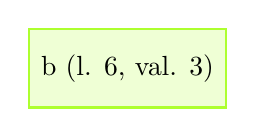
\begin{tikzpicture}
        \node[CasePile](1)at(0,0){\Code{b} (l. 6, val. \Code{3})};
    \end{tikzpicture}}
    &
    \scalebox{.45}{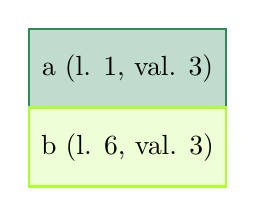
\begin{tikzpicture}
        \node[CasePile,draw=SeaGreen,fill=SeaGreen!30](1)at(0,0)
            {\Code{a} (l. 1, val. \Code{3})};
        \node[CasePile](2)at(0,-1){\Code{b} (l. 6, val. \Code{3})};
    \end{tikzpicture}}
    &
    \scalebox{.45}{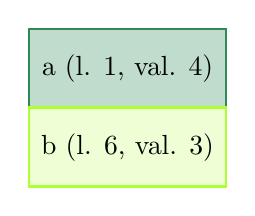
\begin{tikzpicture}
        \node[CasePile,draw=SeaGreen,fill=SeaGreen!30](1)at(0,0)
            {\Code{a} (l. 1, val. \Code{4})};
        \node[CasePile](2)at(0,-1){\Code{b} (l. 6, val. \Code{3})};
    \end{tikzpicture}} \\
    l. 8 & l. 1 & l. 2
    \end{tabular}
\end{flushleft}
\begin{flushleft}
    \begin{tabular}{cc}
    \scalebox{.45}{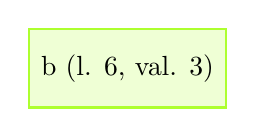
\begin{tikzpicture}
        \node[CasePile](1)at(0,0){\Code{b} (l. 6, val. \Code{3})};
    \end{tikzpicture}}
    &
    \scalebox{.45}{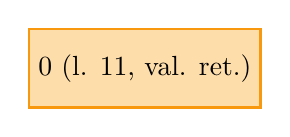
\begin{tikzpicture}
        \node[CasePile,draw=YellowOrange,fill=YellowOrange!30](1)at(0,0)
            {\Code{0} (l. 11, val. ret.)};
    \end{tikzpicture}} \\
    l. 10 & l. 11 
    \end{tabular}
\end{flushleft}
\end{multicols}
\end{frame}

%%%%%%%%%%%%%%%%%%%%%%%%%%%%%%%%%%%%%%%%%%%%%%%%%%%%%%%%%%%%%%%%%%%%%%%%
\begin{frame} \frametitle{Pile}
Les \alert{variables locales} d'une fonction (c.-à-d. les variables déclarées
dans le corps de la fonction) se situent dans la \alert{pile}.
\medskip

De plus, la \alert{valeur renvoyée} (si son type de retour n'est pas 
\Code{void}) se situe dans la \alert{pile}.
\medskip

\uncover<2->{
Après avoir appelé une fonction, c.-à-d. juste après avoir renvoyé
la valeur de retour, la pile se trouve dans le même état qu'avant l'appel.
\bigskip
\bigskip}

\uncover<3->{
{\bf Conséquence très importante}~: toute variable locale à une fonction
est non seulement invisible mais n'existe plus en mémoire hors de la
fonction et après son appel.}
\end{frame}

%%%%%%%%%%%%%%%%%%%%%%%%%%%%%%%%%%%%%%%%%%%%%%%%%%%%%%%%%%%%%%%%%%%%%%%%
\begin{frame}[fragile] \frametitle{Pile}
P.ex., 
\begin{multicols}{2}
\begin{lstlisting}
void fct_1(int a) {
    int b, c;
    b = 1;
    c = 2;
    a = b + c;
}


void fct_2() {
    int x;
    x = 16;
    fct_1(x);
    printf("%d\n", x);
}
...
fct_2();

\end{lstlisting}
\end{multicols}

Configurations de pile~:
\begin{center} \small
\begin{tabular}{cccccccc}
    $\emptyset$
    &
    \scalebox{.45}{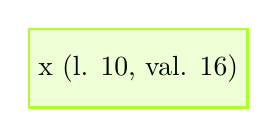
\begin{tikzpicture}
        \node[CasePile](1)at(0,0){\Code{x} (l. 10, val. \Code{16})};
    \end{tikzpicture}}
    &
    \scalebox{.45}{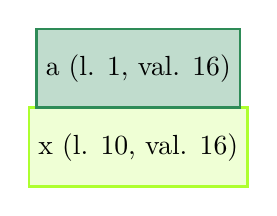
\begin{tikzpicture}
        \node[CasePile](1)at(0,0){\Code{x} (l. 10, val. \Code{16})};
        \node[CasePile,draw=SeaGreen,fill=SeaGreen!30](2)at(0,1)
            {\Code{a} (l. 1, val. \Code{16})};
    \end{tikzpicture}}
    &
    \scalebox{.45}{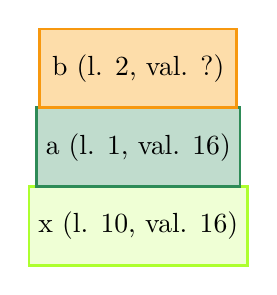
\begin{tikzpicture}
        \node[CasePile](1)at(0,0){\Code{x} (l. 10, val. \Code{16})};
        \node[CasePile,draw=SeaGreen,fill=SeaGreen!30](2)at(0,1)
            {\Code{a} (l. 1, val. \Code{16})};
        \node[CasePile,draw=YellowOrange,fill=YellowOrange!30](3)at(0,2)
            {\Code{b} (l. 2, val. \Code{?})};
    \end{tikzpicture}}
    &
    \scalebox{.45}{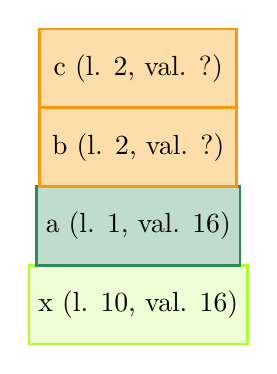
\begin{tikzpicture}
        \node[CasePile](1)at(0,0){\Code{x} (l. 10, val. \Code{16})};
        \node[CasePile,draw=SeaGreen,fill=SeaGreen!30](2)at(0,1)
            {\Code{a} (l. 1, val. \Code{16})};
        \node[CasePile,draw=YellowOrange,fill=YellowOrange!30](3)at(0,2)
            {\Code{b} (l. 2, val. \Code{?})};
        \node[CasePile,draw=YellowOrange,fill=YellowOrange!30](4)at(0,3)
            {\Code{c} (l. 2, val. \Code{?})};
    \end{tikzpicture}}
    &
    \scalebox{.45}{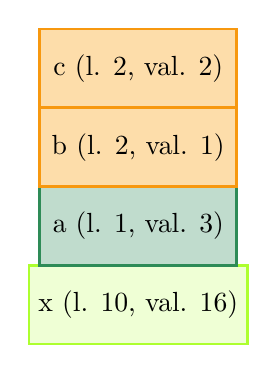
\begin{tikzpicture}
        \node[CasePile](1)at(0,0){\Code{x} (l. 10, val. \Code{16})};
        \node[CasePile,draw=SeaGreen,fill=SeaGreen!30](2)at(0,1)
            {\Code{a} (l. 1, val. \Code{3})};
        \node[CasePile,draw=YellowOrange,fill=YellowOrange!30](3)at(0,2)
            {\Code{b} (l. 2, val. \Code{1})};
        \node[CasePile,draw=YellowOrange,fill=YellowOrange!30](4)at(0,3)
            {\Code{c} (l. 2, val. \Code{2})};
    \end{tikzpicture}}
    &
    \scalebox{.45}{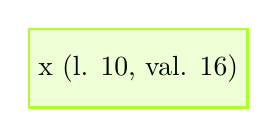
\begin{tikzpicture}
        \node[CasePile](1)at(0,0){\Code{x} (l. 10, val. \Code{16})};
    \end{tikzpicture}}
    &
    $\emptyset$ \\
    l. 15 & l. 11 & l. 2 & l. 3 & l. 3 & l. 6 & l. 13 & l. 17
\end{tabular}
\end{center}
\end{frame}

%%%%%%%%%%%%%%%%%%%%%%%%%%%%%%%%%%%%%%%%%%%%%%%%%%%%%%%%%%%%%%%%%%%%%%%%
\begin{frame}[fragile] \frametitle{Pile et fonctions récursives}
Soit la fonction 
\begin{lstlisting}
void fibo(int a) {
    if (a <= 1) 
        return a;
    return fibo(a - 1) + fibo(a - 2);
}
\end{lstlisting}
et la suite d'instructions
\begin{lstlisting}
int x;
x = fibo(4);
\end{lstlisting}

\begin{center}
    \todo{Dessiner l'arbre des appels et la pile au fur et à mesure 
    de l'exécution.}
\end{center}
\end{frame}

%%%%%%%%%%%%%%%%%%%%%%%%%%%%%%%%%%%%%%%%%%%%%%%%%%%%%%%%%%%%%%%%%%%%%%%%
\begin{frame}[fragile]\frametitle{Fonctions à effet de bord}
Une {\bf fonction} est à \alert{effet de bord} s'il existe au
moins un jeu d'arguments qui fait que l'évaluation de l'appel
à la fonction sur ce jeu d'arguments modifie la mémoire par rapport
à son état d'avant l'appel.
\bigskip

\begin{multicols}{2}
\begin{semiverbatim}\uncover<2->{
inf f(int a, int b) \{
    return 21 * a + b;
\}}
\end{semiverbatim}
\uncover<2->{
Cette fonction n'est pas à effet de bord. Elle renvoie une valeur
sans modifier la mémoire.}
\end{multicols}
\medskip

\begin{multicols}{2}
\begin{semiverbatim}\uncover<3->{
float double_val(float *x) \{
    *x = 2 * (*x);
    return *x;
\}}
\end{semiverbatim}
\uncover<3->{
Cette fonction est à effet de bord puisqu'elle modifie
une zone de la mémoire (celle à l'adresse spécifiée
par son argument).}
\end{multicols}
\end{frame}

%%%%%%%%%%%%%%%%%%%%%%%%%%%%%%%%%%%%%%%%%%%%%%%%%%%%%%%%%%%%%%%%%%%%%%%%
\begin{frame}[fragile]\frametitle{Fonctions à effet de bord}
\begin{multicols}{2}
\begin{semiverbatim}
int g(char c) \{
    int b;
    b = 5;
    return b + c;
\}
\end{semiverbatim}
\uncover<2->{
Cette fonction n'est pas à effet de bord. La déclaration (et l'affectation)
de \Code{b} reste locale à la fonction. Après tout appel à \Code{g},
la variable \Code{b} n'existe plus.}
\end{multicols}

\begin{multicols}{2}
\begin{semiverbatim}\small\uncover<3->{
char *allouer(int n) \{
    char *res;
    res = (char *)
    malloc(sizeof(char) * n);
    return res;
\}}
\end{semiverbatim}
\uncover<4->{
Cette fonction est à effet de bord. Elle réserve en effet,
par l'appel interne à la fonction \Code{malloc}, une zone
de la mémoire, ce qui modifie son état.}
\end{multicols}

\begin{multicols}{2}
\begin{semiverbatim}\small\uncover<5->{
int h(int a, int b) \{
    if (a * b == 0)
        printf("z\\n");
    return a - b;
\}}
\end{semiverbatim}
\uncover<6->{
Cette fonction est à effet de bord. En effet, l'appel à \Code{h}
avec, p.ex., les arguments \Code{1} et \Code{0} provoque un
affichage sur la sortie standard, modifiant l'état de la
mémoire.}
\end{multicols}
\end{frame}

%%%%%%%%%%%%%%%%%%%%%%%%%%%%%%%%%%%%%%%%%%%%%%%%%%%%%%%%%%%%%%%%%%%%%%%%
%%%%%%%%%%%%%%%%%%%%%%%%%%%%%%%%%%%%%%%%%%%%%%%%%%%%%%%%%%%%%%%%%%%%%%%%
\subsection{Commandes préprocesseur}

%%%%%%%%%%%%%%%%%%%%%%%%%%%%%%%%%%%%%%%%%%%%%%%%%%%%%%%%%%%%%%%%%%%%%%%%
\begin{frame} \frametitle{Commandes préprocesseur}
Une \alert{commande préprocesseur} (ou directive préprocesseur) est
une ligne qui commence par \Code{\#}.
\bigskip

\uncover<2->{
Le \alert{préprocesseur} est une unité qui intervient lors de la
compilation. Son rôle est de traiter les commandes préprocesseur.
\medskip

Il fonctionne en construisant une nouvelle version du programme
en {\bf remplaçant} chaque commande préprocesseur par des expressions
en {\sf C} adéquates.
\bigskip}

\uncover<3->{
Il existe plusieurs sortes de commandes préprocesseur~:

\begin{itemize}
    \item les inclusions de fichiers~;
    \smallskip

    \item les définitions de symboles~;
    \smallskip

    \item les macro-instructions à paramètres;
    \smallskip
    
    \item les macro-instructions de contrôle de compilation.
\end{itemize}}
\end{frame}

%%%%%%%%%%%%%%%%%%%%%%%%%%%%%%%%%%%%%%%%%%%%%%%%%%%%%%%%%%%%%%%%%%%%%%%%
\begin{frame}[fragile] \frametitle{Inclusions de fichiers}
La commande préprocesseur
\begin{center}
    \Code{\#include <NOM.h>}
\end{center}
permet d'\alert{inclure} le fichier \Code{NOM.h} dans le programme pour
bénéficier des fonctionnalités qu'il apporte.
\medskip

\uncover<2->{
Le préprocesseur résout cette commande en recopiant le contenu de
\Code{NOM.h} à l'endroit où elle est invoquée.
\bigskip}

\uncover<3->{
Il est possible d'enchaîner les inclusions~:}
\begin{semiverbatim}\uncover<3->{
#include <stdio.h>
#include <stdlib.h>
#include <string.h>}
\end{semiverbatim}
\bigskip

\uncover<4->{
Habituellement, les inclusions sont réalisées au début du programme.}
\end{frame}

%%%%%%%%%%%%%%%%%%%%%%%%%%%%%%%%%%%%%%%%%%%%%%%%%%%%%%%%%%%%%%%%%%%%%%%%
\begin{frame}[fragile] \frametitle{Définitions de symboles}
La commande préprocesseur
\begin{center}
    \Code{\#define SYMB EXP}
\end{center}
permet de \alert{définir un alias} \Code{SYMB} pour l'expression
\Code{EXP}. Ceci autorise à faire référence à l'expression \Code{EXP} par
l'intermédiaire du symbole \Code{SYMB}.
\medskip

\uncover<2->{
Le préprocesseur résout tout invocation \Code{SYMB} en la remplaçant
par \Code{EXP}.
\bigskip}

\uncover<3->{
À gauche (resp. à droite), des instructions avant (resp. après) le
passage du préprocesseur~:}
\begin{multicols}{2}
\begin{semiverbatim}\small\uncover<3->{
#define NB 5
#define CHAINE "cba\\n"
...
for (i = 1 ; i <= NB ; ++i) \{
    printf("%s", CHAINE);
\}}
\end{semiverbatim}
\begin{semiverbatim}\small\uncover<3->{
/* Rien. */
/* Rien. */
...
for (i = 1 ; i <= 5 ; ++i) \{
    printf("%s", "cba\\n");
\}}
\end{semiverbatim}
\end{multicols}

\uncover<4->{
Par convention, tout alias est constitué de lettres majuscules,
de chiffres ou de tirets bas.}
\end{frame}

%%%%%%%%%%%%%%%%%%%%%%%%%%%%%%%%%%%%%%%%%%%%%%%%%%%%%%%%%%%%%%%%%%%%%%%%
\begin{frame}[fragile] \frametitle{Macro-instructions à paramètres}
La commande préprocesseur
\begin{center}
    \Code{\#define SYMB(P1, P2, ..., Pn) EXP}
\end{center}
permet de définir une \alert{macro-instruction à paramètres} \Code{SYMB}.
Ceci autorise à faire référence à l'expression \Code{EXP} par
l'intermédiaire du symbole \Code{SYMB} paramétrable par des
paramètres \Code{P1}, \Code{P2}, \dots, \Code{Pn}.
\medskip

\uncover<2->{
Le préprocesseur résout toute invocation \Code{SYMB(A1, A2, ..., An)}
en la remplaçant par l'expression obtenue en substituant \Code{Ai}
à toute occurrence du paramètre \Code{Pi} dans \Code{EXP}.
\bigskip}

\uncover<3->{
À gauche (resp. à droite), des instructions avant (resp. après) le
passage du préprocesseur~:}
\begin{multicols}{2}
\begin{semiverbatim}\small\uncover<3->{
#define MAX(a, b) a > b ? a : b
...
int x;
x = MAX(10, 14);}
\end{semiverbatim}
\begin{semiverbatim}\small\uncover<3->{
/* Rien. */
...
int x;
x = 10 > 14 ? 10 : 14;}
\end{semiverbatim}
\end{multicols}
\end{frame}

%%%%%%%%%%%%%%%%%%%%%%%%%%%%%%%%%%%%%%%%%%%%%%%%%%%%%%%%%%%%%%%%%%%%%%%%
\begin{frame}[fragile] \frametitle{Macro-instructions à paramètres}
{\bf Problème}~: étudions comment le préprocesseur transforme les
instructions suivantes~:
\begin{semiverbatim}
#define CARRE(a) a * a
...
x = 2;
y = 3;
z = CARRE(x + y);
\end{semiverbatim}
\uncover<2->{
La l. 5 est remplacée par \Code{z = x + y * x + y;}.

Ainsi, la valeur \Code{2 + 3 * 2 + 3 = 13} est affectée à \Code{z} au
lieu de \Code{25} comme attendu.
\bigskip}

\uncover<3->{
{\bf Solution}~: il faut placer des parenthèses autour des paramètres
des macro-instructions à paramètres~:}
\begin{semiverbatim}\uncover<3->{
#define CARRE(a) (a) * (a)}
\end{semiverbatim}
\uncover<4->{
De cette façon, \Code{CARRE(x + y)} est remplacée par
\Code{(x + y) * (x + y)} comme désiré.}
\end{frame}

%%%%%%%%%%%%%%%%%%%%%%%%%%%%%%%%%%%%%%%%%%%%%%%%%%%%%%%%%%%%%%%%%%%%%%%%
\begin{frame}[fragile] \frametitle{Macro-instructions à paramètres}
{\bf Problème}~: étudions comment le préprocesseur transforme les
instructions suivantes~:
\begin{semiverbatim}
#define DOUBLE(a) (a) + (a)
...
x = 3;
z = 5 * DOUBLE(x);
\end{semiverbatim}
\uncover<2->{
La l. 4 est remplacée par \Code{z = 5 * (x) + (x);}.

Ainsi, la valeur \Code{5 * 3 + 3 = 18} est affectée à \Code{z} au lieu de
\Code{30} comme attendu.
\bigskip}

\uncover<3->{
{\bf Solution}~: il faut placer des parenthèses autour de l'expression
toute entière~:}
\begin{semiverbatim}\uncover<3->{
#define DOUBLE(a) ((a) + (a))}
\end{semiverbatim}
\uncover<4->{
De cette façon, \Code{5 * DOUBLE(x)} est remplacée par
\Code{5 * ((x) + (x))} comme désiré.}
\end{frame}

%%%%%%%%%%%%%%%%%%%%%%%%%%%%%%%%%%%%%%%%%%%%%%%%%%%%%%%%%%%%%%%%%%%%%%%%
\begin{frame} \frametitle{Macro-instructions de contrôle de compilation}
Les \alert{macro-instructions de contrôle de compilation} permettent 
d'ignorer, lors de la compilation, une partie du programme.
\medskip

Ceci est utile pour {\bf sélectionner} les parties à prendre en compte 
dans un programme, sans avoir à les (dé)commenter.
\bigskip

On dispose ainsi des constructions
\begin{multicols}{3}
\Code{\#ifdef SYMB} \\
\Code{\dots} \\
\Code{\#endif}
\bigskip
\bigskip

\Code{\#ifndef SYMB} \\
\Code{\dots} \\
\Code{\#endif}
\bigskip
\bigskip

\Code{\#ifdef SYMB} \\
\Code{\dots} \\
\Code{\#else} \\
\Code{\dots} \\
\Code{\#endif}
\end{multicols}

À gauche, le code \Code{\dots} n'est considéré que si l'alias \Code{SYMB}
est défini.
\medskip

Au centre, le code \Code{\dots} n'est considéré que si l'alias \Code{SYMB}
n'est pas défini.
\end{frame}

%%%%%%%%%%%%%%%%%%%%%%%%%%%%%%%%%%%%%%%%%%%%%%%%%%%%%%%%%%%%%%%%%%%%%%%%
\begin{frame}[fragile] 
\frametitle{Macro-instructions de contrôle de compilation}
\begin{multicols}{2}
\begin{lstlisting}[basicstyle=\ttfamily\scriptsize]
#include <stdio.h>


#define GAUCHE_DROITE

#ifdef GAUCHE_DROITE

int rechercher(char *tab, 
        int n, char x) {
    int i;
    for (i = 0 ; i <= n ; ++i)
        if (tab[i] == x)
            return i;
    return -1;
}

#else


int rechercher(char *tab, 
        int n, char x) {
    int i;
    for (i = n - 1 ; i >= 0 ; --i)
        if (tab[i] == x)
            return i;
    return -1;
}

#endif

int main() {
    int res;
    char tab[] = "chaine de test";
    
    res = rechercher(tab, 14, 't');
    printf("%d\n", res);
}
\end{lstlisting}
\end{multicols}

\begin{footnotesize}
Ici, on donne deux algorithmes pour localiser la première occurrence
d'une lettre dans un tableau~: de la gauche vers la droite, ou bien
de la droite vers la gauche.
\smallskip

Ce programme affiche \Code{10}~; si on renomme \Code{GAUCHE\_DROITE}
(en l. 4), il affiche \Code{13}.
\end{footnotesize}
\end{frame}
